\documentclass[conference]{IEEEtran}

% ========= 日本語対応(LuaLaTeX推奨) =========
\usepackage{luatexja}
\usepackage{luatexja-fontspec}
\setmainjfont{HaranoAjiMincho}
\setsansjfont{HaranoAjiGothic}

% ========= 一般パッケージ =========
\usepackage{amsmath,amssymb}
\usepackage{graphicx}
\usepackage{booktabs}
\usepackage{array}
\usepackage{url}
\usepackage[hidelinks]{hyperref}
\usepackage{cite}

% ========= 図・グラフ =========
\usepackage{tikz}
\usetikzlibrary{arrows.meta,decorations.pathreplacing,calc,patterns}
\usepackage{pgfplots}
\pgfplotsset{compat=1.17}

% ========= タイトル =========
\title{DRAM技術導入とその戦略的位置づけ(1997--2001)\\
\large 酒田FabにおけるDRAM/PSRAMとロジック展開の関連}

\author{%
  \IEEEauthorblockN{三溝 真一 (Shinichi Samizo)}%
  \IEEEauthorblockA{独立系半導体研究者(元セイコーエプソン)\\%
  Independent Semiconductor Researcher (ex-Seiko Epson)\\%
  Email: \href{mailto:shin3t72@gmail.com}{shin3t72@gmail.com}\\%
  GitHub: \url{https://github.com/Samizo-AITL}}%
}

\begin{document}
\maketitle

\begin{abstract}
\textbf{(日本語)}\\
本論文は,1997年から2001年にかけてセイコーエプソン酒田事業所が
三菱電機からの技術移管を通じて \mbox{0.5\,$\mu$m} $\rightarrow$ \mbox{0.35\,$\mu$m} $\rightarrow$ \mbox{0.25\,$\mu$m} の
DRAMプロセスを短期間で習得し,得られたプロセス知見を
先端ロジック,高耐圧混載CMOSへ展開して液晶ドライバー製品化に結びつけた
技術的・戦略的過程を,筆者の実体験に基づき整理する。
主要な不良モード(Pause/Disturb Refresh)の物理起源と対策,
および量産歩留まりの推移を示し,獲得した知見がその後の
事業ドメインへどのように接続されたかを考察する。\\[1ex]

\textbf{(English)}\\
This paper reviews 1997–2001, when Seiko Epson’s Sakata Fab
assimilated DRAM processes (0.5\,$\mu$m → 0.35\,$\mu$m → 0.25\,$\mu$m) transferred from Mitsubishi Electric.
The acquired know-how was extended beyond DRAM to advanced logic
and high-voltage mixed CMOS, leading to LCD driver products.
Key failure modes (Pause/Disturb Refresh), countermeasures, and yield evolution
are summarized based on the author’s on-site experience.
\end{abstract}

\begin{IEEEkeywords}
DRAM, VSRAM/PSRAM, 0.25\,$\mu$m process, retention failure, disturb failure, Sakata Fab, technology transfer, high-voltage mixed CMOS, LCD driver, process learning

\hspace{1em}(日本語)DRAM,VSRAM/PSRAM,0.25\,$\mu$mプロセス,リテンション不良,ディスターブ不良,酒田Fab,技術移管,高耐圧混載CMOS,液晶ドライバー,プロセス習得
\end{IEEEkeywords}

\section{序論}
1997年,当時の半導体産業は \textit{Windows~95} の世界的普及や
Intel Pentium~II の登場を契機として急成長局面にあった。
製造技術面では,8インチウェーハラインと 0.35\,$\mu$m 世代プロセスの
量産化が進展し,DRAM およびロジックLSIの分野で国際競争が一層激化していた。

セイコーエプソンは,山形県酒田市に新たに建設した 8インチFab
(酒田事業所)において,三菱電機からの技術移管を通じて
0.5\,$\mu$m $\rightarrow$ 0.35\,$\mu$m $\rightarrow$ 0.25\,$\mu$m
の三世代DRAMプロセスを短期間で習得した。
しかしその狙いは,必ずしもDRAM事業で競争優位を確立することではなく,
むしろDRAMを媒体として最新プロセスを自前化し,
最終的にはロジック/高耐圧混載CMOSや液晶ドライバーに展開する点にあった。

本研究は,この「DRAM導入を目的ではなく手段とする」戦略的枠組みを,
筆者の現場経験に基づき実証的に整理するものである。
特に,立ち上げ初期の不良モード解析(Pause/Disturb Refresh Fail)とその対策,
歩留まり改善プロセス,さらに獲得知見がロジック展開に
どのように接続されたかを考察する。

\section{第1章:0.5\,\texorpdfstring{$\mu$m}{μm} と 0.35\,\texorpdfstring{$\mu$m}{μm} 世代の立ち上げ}

\subsection{0.5\,$\mu$m 16M DRAM}
酒田Fabにおける最初の量産製品は,0.5\,$\mu$m世代の16M DRAMであった。
この製品は熊本Fabで確立されたプロセスを移管したものであり,
設備条件やプロセスレシピの親和性が高く,比較的スムーズに立ち上がった。
\begin{itemize}
  \item 熊本で実績のある16M DRAMプロセスを導入
  \item 酒田Fabの8インチ設備との適合性が良好
  \item 初期歩留まりから安定しており,短期間で量産に到達
\end{itemize}

\subsection{0.35\,$\mu$m 64M DRAM:洗浄フロー差異と「鏡写し」}
\subsubsection{初期の困難}
1997年秋,試作ロットを30ロット以上投入したが,いずれも
パターン形状が大きく崩れ,SEM観察で寸法測定すら困難な状況であった。

\subsubsection{原因究明}
徹底調査の結果,問題はプロセスの本質的差異ではなく,
\emph{洗浄フローのわずかな違い}に起因していたことが判明した。
熊本は「硫酸過水→アンモニア過水→塩酸過水」,酒田は効率化で
「アンモニア過水→塩酸過水」(硫酸過水省略)であった。

\subsubsection{解決と「鏡写し」}
熊本プロセスをフロー・装置条件まで\emph{完全鏡写し}で再現し解消。
この経験が次世代0.25\,$\mu$mの土台となった。

\subsection{小括}
0.5\,$\mu$mは忠実移管で量産性を確立。0.35\,$\mu$mは洗浄差異が原因,
鏡写し徹底で回復。

\section{第2章:0.25\,\texorpdfstring{$\mu$m}{μm} 世代64M DRAMの立ち上げ}
\subsection{SCF方式と初期歩留まり}
\emph{Short Cycle Feedback (SCF)} を0.5\,$\mu$m時から継続採用。
短サイクルで評価・FBし工程を最適化。初期本番で約65\%に到達。
\begin{enumerate}
  \item 移管条件を流動票に展開
  \item 主要工程で途中止め・形状確認(約10ロット)
  \item SEM/電気評価で条件修正
  \item 本番3ロットを通し信頼性確認
\end{enumerate}

\subsection{保持時間モデルと不良モード解析}
初期不良は \emph{Pause Refresh Fail} に集中。32→64→128\,msで単ビット不良が散発増。
ライン欠陥・エッジ集中はなくランダム(Fig.~\ref{fig:failmap})。

\begin{equation}
\tau=\frac{C_{\mathrm{cell}}\cdot V_{\mathrm{cell}}}{I_{\mathrm{leak}}}
\end{equation}
設計通りの $C_{\mathrm{cell}}$,$V_{\mathrm{cell}}$ に対し,$I_{\mathrm{leak}}$ 増大が課題。
キャパ誘電体/構造欠陥は否定,\emph{拡散層ジャンクションリーク} を特定。
物理起源の概念は Fig.~\ref{fig:dram_cross_section}。

\begin{figure}[t]\centering
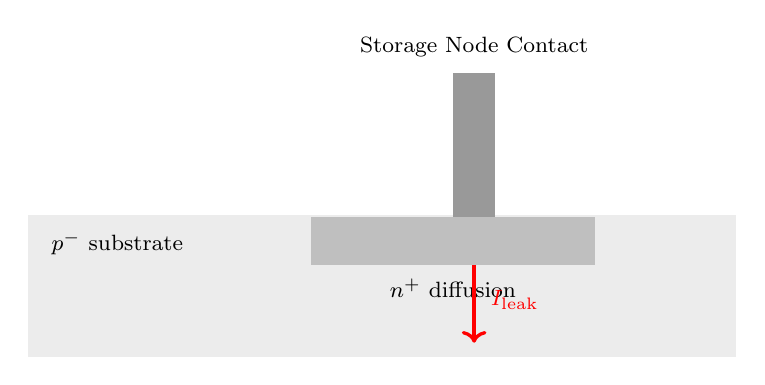
\begin{tikzpicture}[scale=1.8]
\fill[gray!15] (-1,0) rectangle (4,-1.0);
\node[anchor=north west] at (-0.9,-0.05) {\footnotesize $p^-$ substrate};
\fill[gray!50] (1,-0.01) rectangle (3,-0.35);
\node[anchor=north] at (2,-0.38) {\footnotesize $n^+$ diffusion};
\fill[black!40] (2,-0.01) rectangle (2.3,1.0);
\node[anchor=south] at (2.15,1.05) {\footnotesize Storage Node Contact};
\draw[->,very thick,red] (2.15,-0.35) -- (2.15,-0.9);
\node[anchor=west,red] at (2.2,-0.6) {\footnotesize $I_{\mathrm{leak}}$};
\end{tikzpicture}
\caption{DRAM セル断面概念(SNコンタクト/$n^+$拡散層/$p^-$基板)。赤矢印が $n^+\!\rightarrow\!p^-$ リーク $I_{\mathrm{leak}}$。}
\label{fig:dram_cross_section}
\end{figure}

\begin{figure}[t]\centering
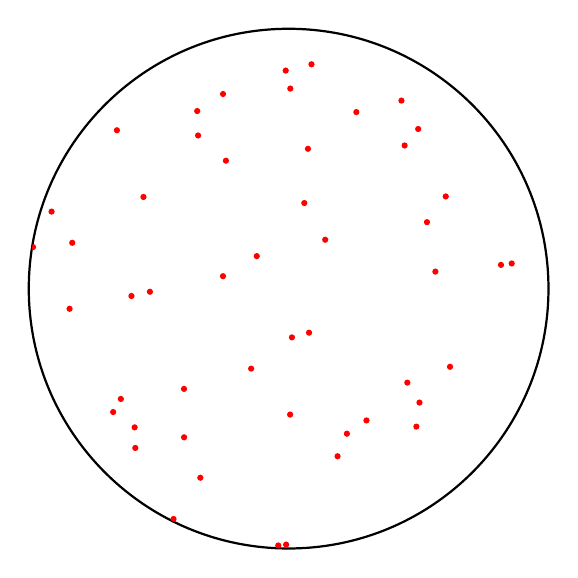
\begin{tikzpicture}[scale=0.22]
  \def\R{15}
  \draw[thick] (0,0) circle (\R);
  \begin{scope}\clip (0,0) circle (\R);
    \foreach \i in {1,...,60}{
      \pgfmathsetmacro{\xx}{(rnd*2-1)*\R}
      \pgfmathsetmacro{\yy}{(rnd*2-1)*\R}
      \fill[red] (\xx,\yy) circle (0.18);
    }
  \end{scope}
\end{tikzpicture}
\caption{Pause Refresh Fail のフェイルビットマップ(ウエハ外周円+ランダム赤点)。}
\label{fig:failmap}
\end{figure}

\subsection{プラズマダメージ仮説}
酸素プラズマ曝露(ゲートエッチ後露出,LDDでの繰返しアッシング)で界面欠陥準位が生成し,熱励起キャリア経由でリーク増大と推定。

\subsection{対策と効果}
レジスト剥離を \emph{O$_2$アッシング→硫酸剥離} に全面切替。感受性の高い工程後のプラズマ曝露をゼロ化し界面欠陥を根絶。
\begin{table}[t]
  \centering
  \caption{レジスト剥離フローの切替(Before/After)}
  \label{tab:resist_flow}
  \begin{tabular}{p{0.25\linewidth} p{0.65\linewidth}}
    \toprule
    従来(Before) & O$_2$アッシングによるドライ剥離 \\
    対策後(After) & 硫酸剥離によるウエット剥離 \\
    主効果 & プラズマ曝露ゼロ化,界面欠陥・ジャンクションリーク抑制 \\
    歩留まり & 65\% $\rightarrow$ 80\%台後半(Pause改善が支配) \\
    \bottomrule
  \end{tabular}
\end{table}

この切替により Pause は大幅減,量産歩留まりは 65\% から 80\%台後半へ改善(Fig.~\ref{fig:yield_trend})。

\begin{figure}[t]\centering
\begin{tikzpicture}
\begin{axis}[
  width=\linewidth,height=6cm,
  ymin=0, ymax=100, ylabel={歩留まり(\%)},
  symbolic x coords={0.5\,\mu m,0.35\,\mu m,0.25\,\mu m,VSRAM},
  xtick=data, xticklabel style={align=center}, xlabel={プロセス世代},
  grid=both, legend style={at={(0.5,-0.28)},anchor=north,draw=none,fill=none},
  legend columns=2, clip=false]
  \addplot+[semithick,mark=*] coordinates {(0.5\,\mu m,95) (0.35\,\mu m,20) (0.25\,\mu m,65) (VSRAM,30)};
  \addlegendentry{初期歩留まり}
  \addplot+[semithick,mark=square*] coordinates {(0.5\,\mu m,95) (0.35\,\mu m,86) (0.25\,\mu m,88) (VSRAM,80)};
  \addlegendentry{改善後}
\end{axis}
\end{tikzpicture}
\caption{酒田Fabにおける世代別歩留まり推移。}
\label{fig:yield_trend}
\end{figure}

\subsection{小括}
SCFで65\%の高い初期歩留まりを確保。主因はジャンクションリークで,プラズマ曝露ゼロ化で80\%台後半に。

\section{第3章:VSRAM(2001年)— Pause/Disturb対策と歩留まり改善}

\subsection{開発背景と初期状況}
モバイル用途の低消費・90\,$^\circ$C高温保証のため,0.25\,$\mu$m DRAMを流用し\emph{VSRAM}を開発。
初期量産は約30\%で出荷優先の厳しい判断。筆者が歩留まり改善を担当。

\subsection{顕在化した不良モード}
\begin{itemize}
  \item \textbf{Pause Refresh Fail}: リフレッシュ停止時に保持不足。
  \item \textbf{Disturb Refresh Fail}: 動作中のワードラインが隣接セルを誤反転。
\end{itemize}

\subsection{物理的要因}
Pause は $I_{\mathrm{junc}}$ 増大で $\tau$ 短縮。Fig.~\ref{fig:pause_temp_junc} に示すように温度で指数増大し,バックバイアス強化で抑制。
Disturb は短チャネル効果(SCE)由来。Fig.~\ref{fig:disturb_temp_sce} に示すように CD短小で $I_{\mathrm{off}}$ が急増,温度依存も強い。

\begin{figure}[t]\centering
\begin{tikzpicture}
\begin{axis}[
  width=\linewidth, height=6cm,
  xlabel={温度 [$^\circ$C]}, ylabel={ジャンクションリーク $I_{\mathrm{junc}}$(相対)},
  ymode=log, ymin=1e-2, ymax=1e2,
  xmin=25, xmax=100, xtick={25,40,60,80,90,100},
  grid=both, legend style={at={(0.5,-0.22)},anchor=north,draw=none,fill=none},
  clip=false]
  \addplot+[semithick,mark=*] coordinates {(25,0.02) (40,0.06) (60,0.3) (80,1.6) (90,3.2) (100,6.0)};
  \addlegendentry{$V_{bs}=-1$\,V}
  \addplot+[semithick,mark=square*] coordinates {(25,0.01) (40,0.03) (60,0.12) (80,0.45) (90,0.9) (100,1.8)};
  \addlegendentry{$V_{bs}=-3$\,V}
\end{axis}
\end{tikzpicture}
\caption{Pause:温度で $I_{\mathrm{junc}}$ は指数増。バックバイアス強化で抑制。}
\label{fig:pause_temp_junc}
\end{figure}

\begin{figure}[t]\centering
\begin{tikzpicture}
\begin{axis}[
  width=\linewidth, height=6cm,
  xlabel={温度 [$^\circ$C]}, ylabel={トランジスタリーク $I_{\mathrm{off}}$(相対)},
  ymode=log, ymin=1e-3, ymax=1e1,
  xmin=25, xmax=100, xtick={25,40,60,80,90,100},
  grid=both, legend style={at={(0.5,-0.22)},anchor=north,draw=none,fill=none},
  clip=false]
  \addplot+[semithick,mark=triangle*] coordinates {(25,0.004) (40,0.01) (60,0.05) (80,0.22) (90,0.45) (100,0.9)};
  \addlegendentry{CD=0.25\,\,$\mu$m}
  \addplot+[semithick,mark=*] coordinates {(25,0.01) (40,0.03) (60,0.15) (80,0.7) (90,1.4) (100,2.8)};
  \addlegendentry{CD=0.20\,\,$\mu$m}
\end{axis}
\end{tikzpicture}
\caption{Disturb:短チャネル効果で $I_{\mathrm{off}}$ 増大。温度依存も強い。}
\label{fig:disturb_temp_sce}
\end{figure}

\subsection{対策と実装}
\begin{itemize}
  \item \textbf{Pause対策}:HF洗浄回数最小化(ゲート酸化膜残膜確保,SN近傍リーク低減)/バックバイアス強化($-1\to-3$\,V)
  \item \textbf{Disturb対策}:ゲートCD中心値の厳格管理/バックバイアス強化/セルのチャネルドーピング増で $V_\mathrm{th}$ 向上
\end{itemize}

\begin{table}[t]
\centering
\caption{Pause / Disturb 不良に対する主な対策}
\begin{tabular}{p{0.18\linewidth} p{0.28\linewidth} p{0.46\linewidth}}
\toprule
不良モード & 主因 & 主な対策 \\
\midrule
Pause   & ジャンクションリーク & HF洗浄制御,バックバイアス強化 \\
Disturb & 短チャネル効果       & CD管理,チャネルドーピング,バックバイアス強化 \\
\bottomrule
\end{tabular}
\end{table}

\subsection{効果と歩留まり推移}
Pause/Disturbともに顕著に低減。歩留まりは30\%→80\%台に回復。

\section{第4章:0.18\,\texorpdfstring{$\mu$m}{μm} トレンチ系の評価と断念}

\subsection{評価対象と背景}
台湾NANYAの0.18\,$\mu$m DRAMプロセス(東芝系トレンチ方式)を用いたVSRAM/PSRAM試作を検討。0.25\,$\mu$m後継として高密度・低消費を狙う。

\subsection{技術的特徴}
\begin{itemize}
  \item \textbf{キャパシタ構造}: トレンチ型で面積効率は高いが,ジャンクション面積が増大しリークが増えやすい。
  \item \textbf{動作仕様}: DRAM標準の80$^\circ$C保証レベルで,モバイル要求の90$^\circ$Cは設計余裕が小さい。
\end{itemize}

\subsection{課題の顕在化}
90$^\circ$Cで Pause/Disturb が顕著化。トレンチはジャンクション面積増に比例して $I_{\mathrm{junc}}$ が増加(Fig.~\ref{fig:trench_area_leak})。

\begin{figure}[t]\centering
\begin{tikzpicture}
\begin{axis}[
  width=\linewidth, height=6cm,
  xlabel={ジャンクション面積(相対)}, ylabel={ジャンクションリーク $I_{\mathrm{junc}}$(相対)},
  xmin=0.5, xmax=2.5, ymin=0, ymax=3.5,
  xtick={0.5,1.0,1.5,2.0,2.5},
  ytick={0,0.5,1.0,1.5,2.0,2.5,3.0},
  grid=both, legend style={at={(0.5,-0.22)},anchor=north,draw=none,fill=none},
  clip=false]
  \addplot+[semithick,mark=square*] coordinates {(0.5,0.25) (1.0,0.5) (1.5,0.8) (2.0,1.1) (2.5,1.4)};
  \addlegendentry{80$^\circ$C}
  \addplot+[semithick,mark=*] coordinates {(0.5,0.5) (1.0,1.0) (1.5,1.6) (2.0,2.2) (2.5,2.9)};
  \addlegendentry{90$^\circ$C}
\end{axis}
\end{tikzpicture}
\caption{トレンチキャパ:面積にほぼ比例して $I_{\mathrm{junc}}$ が増加。高温ほど増加率が大きい。}
\label{fig:trench_area_leak}
\end{figure}

\subsection{評価結果と戦略判断}
NANYA 0.18\,$\mu$mではモバイル必須の90$^\circ$C保証が満たせないと判断。
次世代VSRAMは断念し,\emph{高耐圧混載CMOS(液晶ドライバー)}へ集中。

\section{結論}
1997–2001年の酒田FabにおけるDRAM導入は,目的ではなく\emph{手段}だった。
移管・鏡写しで確実に立ち上げ,SCFで0.25\,$\mu$mを短期立ち上げ。
Pauseの主因はジャンクションリークで,\emph{O$_2$アッシング→硫酸剥離}への切替で80\%台後半まで改善。
モバイル要求下のVSRAMではPause/Disturbが顕在化したが,
HF洗浄制御・バックバイアス強化・CD管理・チャネルドーピングで歩留まりを30\%→80\%台へ。
一方,0.18\,$\mu$mトレンチは高温保持で限界が明確となり,事業は液晶ドライバーにフォーカスした。
DRAMで得た先端プロセス知見は,最終的に高耐圧混載CMOSで競争力の核となった。

\section*{参考文献}
\begin{thebibliography}{00}
\bibitem{sze2006psd} S.~M.~Sze and K.~K.~Ng, \emph{Physics of Semiconductor Devices}, 3rd ed., Wiley, 2006.
\bibitem{tanaka1996dramtrends} T.~Tanaka et al., ``Trends and Challenges in DRAM Scaling,'' \emph{IEEE JSSC}, 31(11), 1615--1624, 1996.
\bibitem{rizzoli2000retention} L.~Rizzoli et al., ``Retention and Disturb Characterization in 0.25\,\textmu m DRAM,'' \emph{Proc. ITC}, 2000.
\bibitem{okhonin1998retention} S.~Okhonin et al., ``Retention Time and Junction Leakage in Deep Submicron DRAM,'' \emph{IEDM Tech. Dig.}, 549--552, 1998.
\bibitem{wong1999dram} H.-S.~P.~Wong, ``Technology and Device Scaling for DRAM,'' \emph{IBM J. R\&D}, 43(1–2), 133--168, 1999.
\bibitem{chang1994plasma} C.~Chang and S.~C.~Lee, ``Plasma-Induced Damage on Gate Oxides,'' \emph{J. Electrochem. Soc.}, 141(9), 2512--2517, 1994.
\bibitem{mosys2001} MoSys Inc., ``1T-SRAM Technology Overview,'' White Paper, 2001.
\bibitem{kim2002psram} J.~Kim et al., ``Low Power Refresh Schemes for Mobile DRAM/PSRAM,'' \emph{Symp. VLSI Circuits}, 190--193, 2002.
\bibitem{schuegraf1997plasma} K.~Schuegraf et al., ``Impact of Plasma Damage on Junction Leakage and Gate Oxide Reliability,'' \emph{VMIC Proc.}, 73--79, 1997.
\end{thebibliography}

\section*{著者略歴}
\noindent\textbf{三溝 真一 (Shinichi Samizo)} は、信州大学大学院 工学系研究科 電気電子工学専攻にて修士号を取得。
セイコーエプソン株式会社に勤務し、半導体ロジック/メモリ/高耐圧インテグレーション、
インクジェット薄膜ピエゾアクチュエータおよび PrecisionCore プリントヘッドの製品化に従事。
現在は独立系半導体研究者として、プロセス/デバイス教育、メモリアーキテクチャ、AIシステム統合等の研究に取り組む。
連絡先: \href{mailto:shin3t72@gmail.com}{shin3t72@gmail.com}

\end{document}
